
\begin{figure}[htbp]
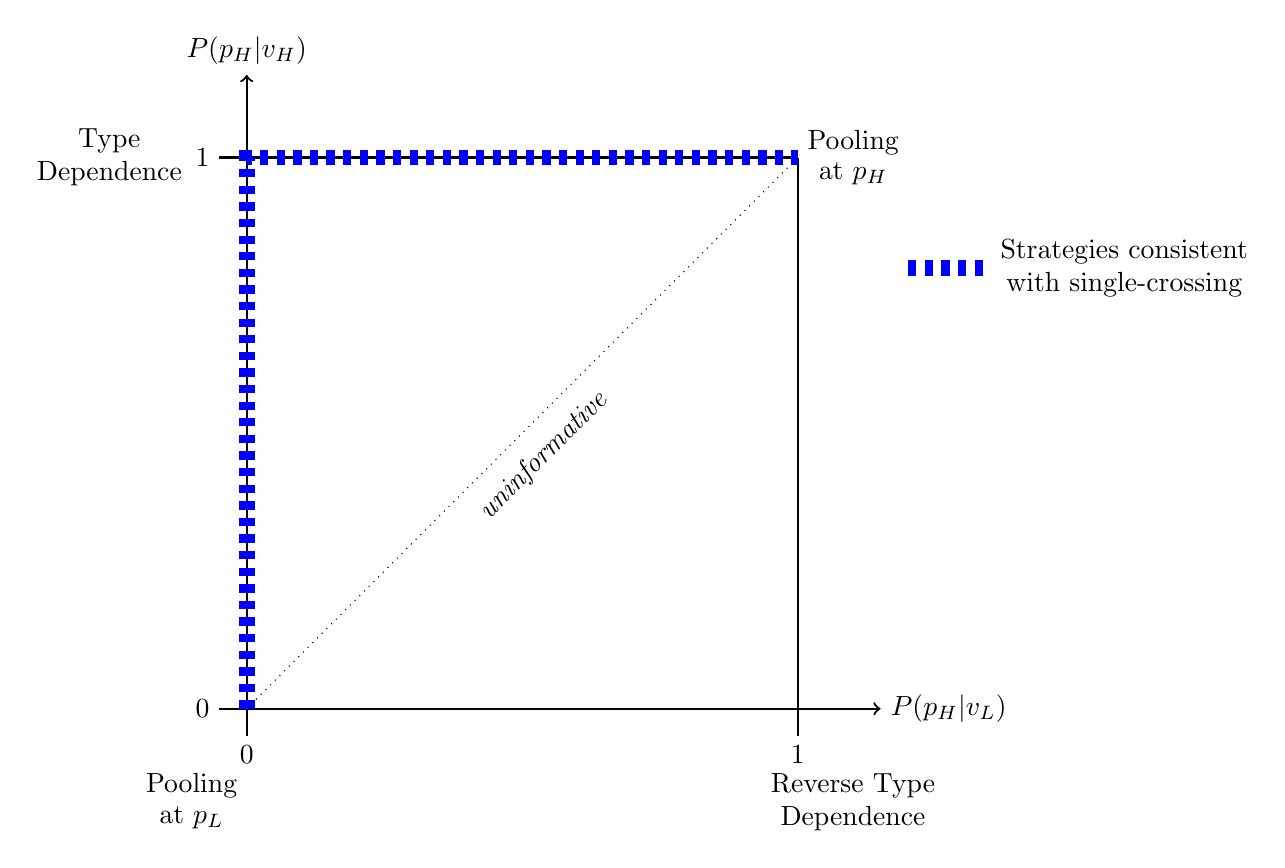
\begin{tikzpicture}[scale=7]

\draw[thick,->] (-0.05,0) -- (1.15,0) node[anchor=west] {$\mathbb{P}(p_H|v_L)$};
\draw[thick,->] (0,-0.05) -- (0,1.15) node[anchor=south] {$\mathbb{P}(p_H|v_H)$};

\draw[thick] (-0.05,1)--(1,1);
\draw[thick] (1,1)--(1,-0.05);

\node[left] at (-0.05,0) {0};
\node[left] at (-0.05,1) {1};
\node[below] at (0,-0.05) {0};
\node[below] at (1,-0.05) {1};

\node[left] at (-0.1,1) {\shortstack{Type \\ Dependence}};
\node[right] at (1,1) {\shortstack{Pooling \\ at $p_H$}};
\node[below] at (1.1,-0.1) {\shortstack{Reverse Type \\ Dependence}};
\node[below] at (-0.1,-0.1) {\shortstack{Pooling \\ at $p_L$}};

\draw[dotted] (0,0)--(1,1);
\coordinate (P) at (0.54,0.46);
\node[rotate=45] (N) at (P) {\emph{uninformative}};

\draw[line width=0.2cm, dashed, blue] (0,0)--(0,1)--(1,1);
\draw[line width=0.2cm, dashed, blue] (1.2,0.8)--(1.35,0.8);
\node[right] at (1.35,0.8) {\shortstack{Strategies consistent \\ with single-crossing}};

\end{tikzpicture}
\caption{Seller Strategy Space}
\label{seller_strat_space}
\end{figure}
